\subsection{Zuk\"unftige Missionen}

Die Analyse des gesamten Datensatzes der beiden Pioneer-Sonden bringt
Klarheit bei Fra\-gen wie, ob die Anomalie auch schon in Erd- oder
Sonnenn\"ahe festgestellt werden kann. Andere R\"atsel k\"onnen nicht
so leicht gel\"ost werden. Um zum Beispiel die Richtung des
Be\-schleunigungsvektors exakt festzustellen oder zu ermitteln in
welchem Bereich genau die Anomalie auftritt, wird eine neue Mission
ben\"otigt. An sie werden bestimmte Anforderun\-gen gestellt\cite{alle2005}\cite{Nieto2004b}\cite{Turyshev2004b}\cite{Nieto2004},
 um den Wert der Beschleunigung genau zu bestimmen
und m\"ogliche Fehlerquellen genau identifizieren und ausschlie{\ss}en
zu k\"onnen.



Das wissenschaftliche Ziel dieser Mission wird sein, die
Pioneer-Anomalie zu best\"atigen und so genau wie m\"oglich zu
erforschen. Ihr Wert soll bis auf mindestens
$10^{-10}\mathit{cm}/s^{2}$ ge\-nau gemessen werden. Es ist
erforderlich eine h\"ohere r\"aumliche und zeitliche Aufl\"osung der
Beschleunigung zu erreichen, um genauere Aussagen \"uber ihre Richtung
und ihren zeitlichen Verlauf machen zu k\"onnen. Interne und externe
Fehlerquellen m\"ussen hierzu genau gepr\"uft und gemessen werden. Es 
ist also auch nötig den Strahlungsdruck der Sonne und
die elektrische Ladung, die sich auf der Oberfl\"ache der
Son\-de ansammelt, genau zu messen. Auf der Mission sollen au{\ss}erdem noch
verschiedene Erkl\"arungsmodelle ge\-testet werden um die Ursache der
Anomalie im Idealfall zu finden. Deshalb wird es auch ein Ziel der Mission sein das newtonsche
Gravitationspotential in gro{\ss}en Entfernungen genau zu bestimmen und
die Bedingungen im tiefen Weltraum zu erforschen. Eine weitere Option
ist die Sonde auf eine Bahn senkrecht zur Ekliptik zu bringen, um
zu \"uberpr\"ufen, wie sich die Anomalie dort verh\"alt.



Um eine Empfindlichkeit f\"ur die Beschleunigungsmessung in Richtung
aller 3 Achsen der Sonde von ca. $10^{-10}\mathit{cm}/s^{2}$ zu
erreichen, ist eine Navigation n\"otig, die pr\"aziser ist, als die der
Pioneers. Daf\"ur ist eine spin-stabilisierte Sonde vorteilhaft. Im
Gegensatz zur 3-Achsen Stabilisation, bereitet das Austreten von
Treibstoff bei der Navigation von spin-stabilisier\-ten Objekten kaum
Probleme. Au{\ss}erdem sind weniger Man\"over zur Korrektur der Lage
notwendig. Bei solchen Ma{\ss}nahmen kann es sein, dass
ungewollt Treibstoff aus\-tritt, was ihre Berechnung enorm erschwert.




Aus den oben genannten Gr\"unden braucht man Korrekturd\"usen,
Kraftstoffleitungen und eine Treibstoffanzeige, die sehr pr\"azise
kalibriert sind, und zus\"atzlich noch genaue Kennt\-nisse \"uber die
zeitliche Entwicklung des Treibstoffverbrauchs. Da diese Informationen
be\-sonders wichtig sind, um die Flugbahn der Sonde m\"oglichst genau
zu bestimmen, werden Sensoren ben\"otigt, die \"uber eine lange Zeit
Daten mit der geforderten Genauigkeit liefern. In diesem Bereich muss
aber noch einiges an Entwicklungsarbeit geleistet werden, da die
Sensoren, die zur Zeit erh\"altlich sind, nicht exakt genug arbeiten
und zu schnell verschlei\-{\ss}en. Eine Echtzeit Anzeige und Kontrolle
ihrer Leistung w\"are au{\ss}erdem noch erw\"unscht.




Die Sonde soll \"ahnlich navigiert werden wie die beiden Pioneer-Sonden,
\"uber Entfernungs- und Geschwindigkeitsbestimmung mit Hilfe von
Radiowellen. Die Entfernung wird \"uber die Laufzeit und die
Geschwindigkeit \"uber die Dopplerverschiebung des Signals ermittelt.
Bei der neuen Mission wird dazu aber nicht nur ein Frequenzband
verwendet, sondern es wird das {\quotedblbase}Dual Band Tracking``
angewendet, welches, wie der Name schon sagt, zwei Fre\-quenzb\"ander
benutzt. Das X-Band (8 -- 12 GHz) und das Ka-Band (26,5 -- 40 GHz) sind
hierf\"ur vorgesehen. Nach M\"oglichkeit sollen noch das
VLBI (Very Long
Baseline Interfe\-rometry) und/oder das $\Delta
$DOR-Verfahren\footnote{Das $\Delta $DOR-Verfahren\cite{delta} funktioniert
so \"ahnlich wie das VLBI. Auch hier wird der Laufzeitunterschied eines
Signals zu zwei weit auseinander stehenden Antennen ermittelt. Dieses
Signal wird dann aber noch mit dem eines Quasars in der N\"ahe der
Sonde abgeglichen, dass einen vergleichbaren Weg zur\"uckgelegt hat.
Die Position des Quasars ist durch vorherige Messungen sehr genau
bekannt. So k\"onnen Fehler, die durch verschiedene St\"orfaktoren, wie
den Sonnenwind oder die Erdatmosph\"are, entstehen, genau ermittelt und
eliminiert werden.} (Delta Differential One-way Ranging) hinzu kommen.
Damit w\"are dann eine genaue Winkelbestimmung m\"oglich, die
ben\"otigt wird um die drei-dimensionalen Beschleunigungsdaten richtig
zu rekonstruieren.


Nat\"urlich muss die Sonde eine interne Energieversorgung haben. Da
diese Mission in den tiefen Weltraum und somit weit weg von der Sonne
f\"uhrt, kommen Solarzellen nicht in\-frage. Noch heute gibt es f\"ur
dieses Problem keine andere L\"osung, als die schon bei den
Pioneer-Sonden verwendeten RTGs. Denn nur diese k\"onnen zuverl\"assig
Energie \"uber einen langen Zeitraum liefern.



Die Platzierung der RTGs stellt eine gro{\ss}e Herausforderung dar, denn
sie emittieren enorm viel Hitze. Um das als Ursache f\"ur die Anomalie
ausschlie{\ss}en zu k\"onnen, sollte die Abstrahlung m\"oglichst
symmetrisch sein. Die RTGs sind aber nicht die einzige W\"arme\-quelle
der Sonde. Auch die Korrekturd\"usen, die verbaute Elektronik und viele
andere Bestandteile emittieren W\"armestrahlung. Diese m\"usste f\"ur
jedes einzelne Bauteil so genau wie m\"oglich untersucht werden.
Seitlich soll die Strahlung durch Abdeckungen abge\-schirmt werden, so
dass sie nur nach vorne oder hinten entweichen kann und ihr
R\"ucksto{\ss} nur in oder entgegen der Flugrichtung wirkt. Dies alles
hilft den drei-dimensionalen Vektor des thermischen R\"ucksto{\ss}es
sehr exakt zu ermitteln. Dazu tragen aber auch alle
reflektierenden Oberfl\"achen der Sonde bei. Deshalb m\"ussten diese
aus Materialien beste\-hen, bei denen vor allem der Alterungsprozess
und die Abstrahleigenschaften sehr genau bekannt sind. Im Idealfall
soll die Sonde so ausbalanciert und symmetrisch konstruiert werden,
dass alle solchen thermischen Einfl\"usse verschwinden.


Eine Neuerung gegen\"uber den Pioneer-Sonden wird sein, dass man an der
neuen Kon\-struktion zwei identische, gegen\"uberliegende Antennen
anbringen wird, die das Radiosi\-gnal gleichzeitig zur Erde und die
entgegengesetzte Richtung absenden. So bleibt die Son\-de in ihrem
Aufbau symmetrisch. Der R\"ucksto{\ss} durch das Senden des Signals
hebt sich auf und muss in der Berechnung nicht mehr ber\"ucksichtigt
werden. Die wichtigste Funktion der Antennen wird aber sein,
zweifelsfrei zu ermitteln ob es sich bei der Anomalie um einen externen
oder internen Effekt handelt. Nachdem pr\"azise Daten der Anomalie mit
einer Orientierung der Antennen aufgenommen wurden, etwa ein bis zwei
Jahre lang, wird die Sonde mit Hilfe von Lichtsensoren, die sich an der
Sonne oder bestimmten Sternen orientieren, um 180{\textdegree} gedreht.
Nun sendet die Antenne, die zuvor nach au{\ss}en gerichtet war, Daten
zur Erde und umgekehrt. Anschlie{\ss}end werden wieder ein bin zwei
Jahre lang pr\"azise Daten aufgenommen und diese dann mit denen der
anderen Antenne verglichen. Stellt man keine Ver\"anderung fest,
best\"atigt dies einen sondenexternen Effekt, \ \"andert sich aber das
Vorzeichen, ist die Ursache sondenintern. Jedes andere Ergebnis, das
von Null verschieden ist, zeigt, dass sowohl ein interner als auch ein
externer Effekt eine Rolle spielen. Ersterer hat dann eine Gr\"o{\ss}e
der H\"alfte der Differenz der beiden Messungen und Letzterer der
H\"alfte der Summe.


\begin{figure}[htnb]
\begin{minipage}[t]{.4\linewidth}
	\centering
	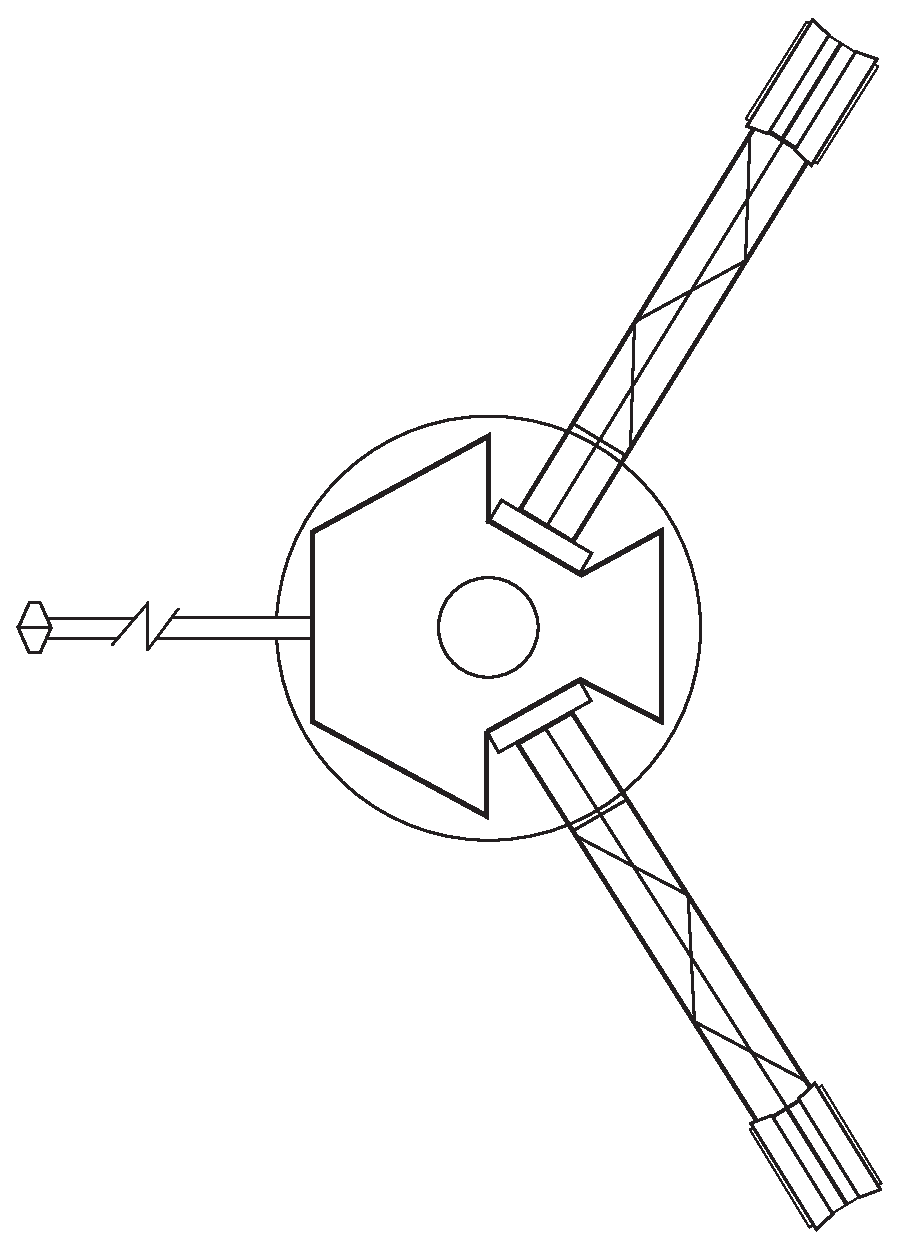
\includegraphics[width=\linewidth]{images/yoyotop}
  \caption{Aufsicht der "Yo-Yo"-Sonde (Skizze)\cite{Nieto2004}}\label{fig:yoyotop}
\end{minipage}
\hfill
\begin{minipage}[t]{.4\linewidth}
	\centering
	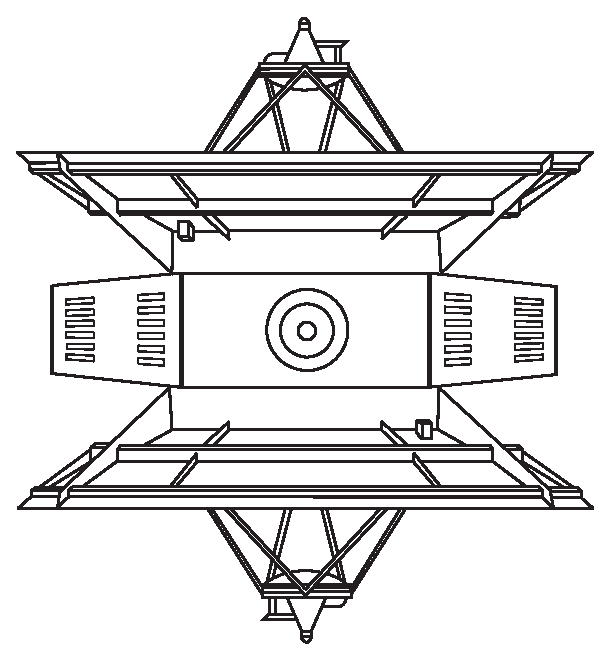
\includegraphics[width=\linewidth]{images/yoyoside}
  \caption{Seitenansicht der "Yo-Yo"-Sonde (Skizze)\cite{Nieto2004}}\label{fig:yoyoside}
\end{minipage}
 \end{figure}

Um das aber tats\"achlich genau so rechnen zu k\"onnen, braucht man
eine komplett symmetrische Sonde wie sie im
{\quotedblbase}Yo-Yo``-Aufbau vorgeschlagen wird. Das Bild zeigt diesen
Aufbau von oben (links) und von der Seite (rechts) in verschiedenen
Ma{\ss}st\"aben. An den beiden langen Auslegern, die in der Draufsicht
gut zu erkennen sind, sollen die RGTs ange\-bracht werden. Die Ausleger sollen
eine L\"ange von 2 -- 2,5 m haben. Je nach dem wie die Mission
endg\"ultig gestaltet wird, kann man an dem dritten Ausleger ein
Instrumentenpaket an\-bringen, um die interstellare Materie
au{\ss}erhalb des Sonnensystems zu erforschen. Zur rei\-nen
Untersuchung der Pioneer-Anomalie, kann man dort auch noch einen dritten
RTG befestigen, was erheblich zur Symmetrie der Sonde beitragen
w\"urde. In der Seitenansicht sind die oben beschriebenen
W\"armeabdeckungen und die Antennen zu sehen. Als Vorlage f\"ur
Letztere wurde die Cassegrain Antenne der Sonde Cassini angepasst.


Eine interessante Modifikation des Aufbaus ist, dass man anstelle der
zweiten Antenne an der Erdabgewandten Seite eine kleine Probemasse
befestigt. Bringt man diese in einem Abstand von {\textgreater} 250 m
von der Sonde an, kann man mit ihrer Hilfe noch eine zweite
Best\"a\-tigung f\"ur die Anomalie erhalten. Die Sonde selbst wird
durch die oben beschriebenen Ra\-diosignale navigiert. Die Bewegung der
Testmasse relativ zur Sonde wird mit Laser-Ab\-standsmessung bestimmt.
Auf diese Weise l\"asst sich die Pioneer-Anomalie zus\"atzlich noch mit
einer zweiten Methode \"uberpr\"ufen.

\begin{figure}[htbn]
\begin{center}
\noindent    
%\psfig{figure=images/lasersonde,width=\linewidth,height=\textheight,keepaspectratio}
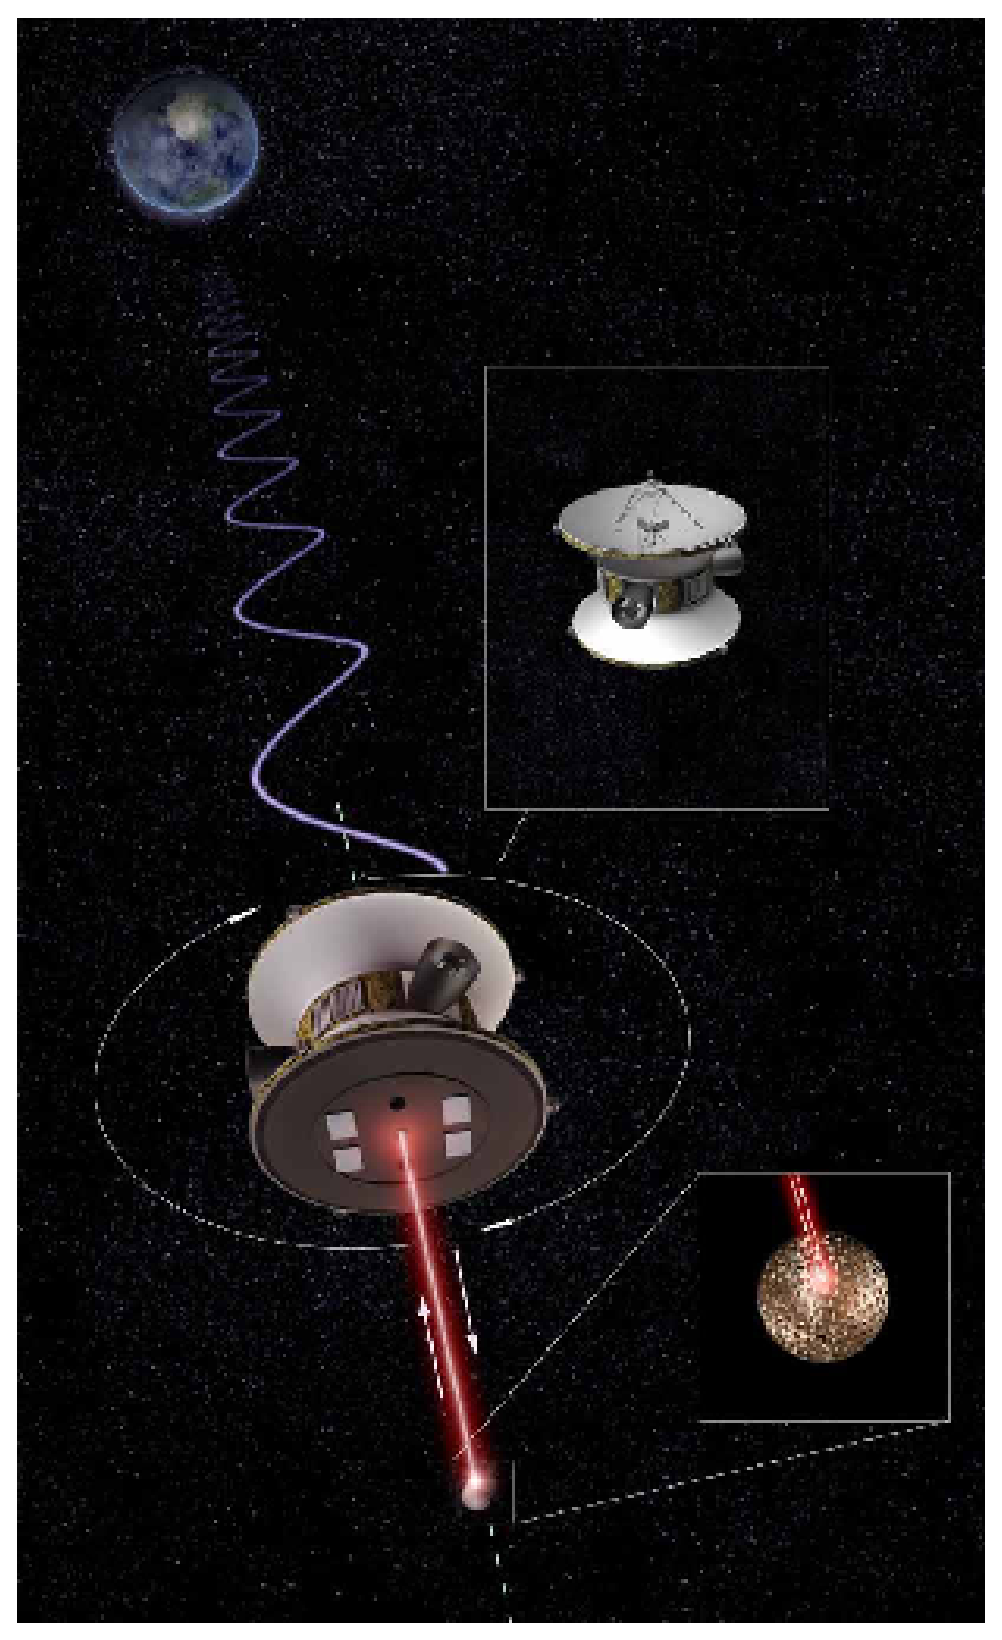
\includegraphics[angle=-90,width=\linewidth]{images/lasersonde}
\end{center}
\vskip -10pt
  \caption{Die Sonde mit zusätzliche Probemasse zur Bestätigung der Pioneer-Anomalie durch Laserabstandsmessung.\cite{alle2005}}
\label{fig:lasersonde}
\end{figure} 


Bei gro{\ss}en Himmelsk\"orpern mit gebundenen und nur wenig
exzentrischen Bahnen konnte die Anomalie nicht festgestellt werden. 
Bei den Pioneer-Sonden wurde sie erst ent\-deckt, als sie sich auf
ihrer hyperbolischen Bahn befanden um das Sonnensystem zu ver\-lassen.
Deshalb und um die Missionsdauer möglichts kurz zu halten, erscheint es sinnvoll 
die Sonde möglichst schnell auf ihre ungebundene Bahn geschickt werden.
Nahe der Sonne sind aber externe systematische Fehler am Experiment, die zum Beispiel 
der Sonnenwind verursacht, sehr groß. Daher ist es sinnvoller die 
Mission etwas zu verlängern und die Sonde erst ab einer Entfernung von mehr als 15
AU auf ihre ungebundene Bahn zu befördern.Da diese Distanz
m\"oglichst schnell erreicht werden soll, wurde f\"ur die Sonde eine
Ge\-schwindigkeit von {\textgreater} 5 - 10 AU/Jahr angedacht. Damit
wird sie wesentlich schneller sein als die beiden Pioneer-Sonden
(Pioneer 10: 2,38 AU/Jahr, Pioneer 11: 2,02 AU/Jahr ). Das dient
zus\"atzlich noch dazu herauszufinden, wie sich die Anomalie bei einer
anderen Ge\-schwindigkeiten verh\"alt und ob eventuell hier ein
Zusammenhang besteht.




Um die gew\"unschte Geschwindigkeit zu erreichen ist ein guter
Antrieb unabk\"ommlich. Mit den heute in der Raumfahrt genutzten
Methoden sind Fluchtgeschwindigkeiten von etwa 5 AU/Jahr m\"oglich. Das
hei{\ss}t, dass beim Start der Sonde eine der existierenden gro{\ss}en
Raketen (Ariane 5, Proton, Delta IV, oder Atlas V) zum Einsatz k\"ame
und im All dann noch einige Flyby-Man\"over zur Beschleunigung
durchgef\"uhrt werden m\"ussten. Die\-ser Missionsverlauf birgt
allerdings einen gro{\ss}en Nachteil. Die ganze Mission w\"urde durch
die Flyby-Man\"over und die geringe Geschwindigkeit zu lange dauern.
Ein Antrieb an Bord der Sonde ist daher unverzichtbar. Etwas passendes
gibt es aber noch nicht. Ein chemischer Antrieb w\"are sehr teuer und
w\"urde an seine Grenzen gebracht werden. Des\-halb werden neue
Technologien entwickelt und getestet. Die Hauptforschungsgebiete sind
ein nuklear-elektrischer, ein solar-elektrischer und ein
solar-thermischer Antrieb. Das gr\"o{\ss}te Interesse, vor allem in
Europa, liegt bei den Solarsegeln. Das ultimative Ziel ist Se\-gel zu
entwickeln, die weniger als $1g/m^{2}$ haben. Da dieses Ziel aber noch
in weiter Fer\-ne liegt, geht der Weg in Richtung vieler Nanor\"ohren
von einigen cm L\"ange, die die Son\-nenenergie nutzbar machen. Mit
einem solchen Segel sind voraussichtlich \ Beschleunigun\-gen auf bis
zu 14 AU/Jahr m\"oglich. Auf H\"ohe der Jupiterbahn wird das Segel dann
abge\-worfen und die eigentliche Mission kann beginnen.




Beim Start hat die Sonde mit allen Bestandteilen eine Gesamtmasse von
ca. 500 kg. Inklu\-sive der beiden Cassegrain Antennen, kommt sie auf
eine Gesamth\"ohe von etwa 3,5 m und auf einen Durchmesser von etwa 2,5
m.




Die Dauer der Mission ist bei einer Geschwindigkeit von 5 AU/Jahr auf 7
Jahre angelegt. In den ersten 3 Jahre wird die Sonde auf eine Distanz
von mehr als 15 AU gebracht. Dort l\"asst der Einfluss der
Sonneneinstrahlung deutlich nach. Die {\quotedblbase}sauberen`` Daten
der letzten 4 Jahre k\"onnen dann genutzt werden um die Anomalie zu
erforschen.Die Lebensdauer der Sonde wird
auf 12 Jahre ausgelegt. Rechnet man mit einer Ge\-schwindigkeit von 10
AU/Jahr, w\"urde die Mission nur 5 Jahre dauern und eine Lebens\-dauer
von 8 Jahren w\"urde gen\"ugen.




Es gibt zwei verschiedene M\"oglichkeiten diese Mission durchzuf\"uhren.
Entweder, wie hier gr\"o{\ss}tenteils beschrieben als eigene Mission,
oder als Teil einer gr\"o{\ss}eren Mission in den tiefen Weltraum.
F\"ur letzteres Konzept gibt es nochmal zwei Versionen. Die eine ist so
ange\-dacht, dass eine Sonde, die zum Beispiel die Bedingungen
au{\ss}erhalb unseres Sonnensys\-tems erforschen soll, mit einem
zus\"atzlichen Instrumentenpaket ausgestattet wird, welches dann die
Anomalie untersuchen soll. Eine anderen Idee ist, dass man eine Sonde
so kon\-struiert, dass auf H\"ohe der Saturnbahn eine Nebensonde von
der Hauptsonde getrennt wird, die dann unabh\"angig von der anderen
Mission die Pioneer-Anomalie erforschen kann. Der Vorteil eines solchen
Szenario ist nat\"urlich, dass es so wesentlich billiger w\"are eine
Sonde ins All zu bef\"ordern und so zus\"atzlich noch andere Bereiche
der Weltraumforschung abgedeckt werden k\"onnen. Die Sonden m\"ussten
daf\"ur aber an zus\"atzliche Anforderungen angepasst werden und
k\"onnten nicht ganz so speziell auf die Erforschung der Anomalie
ausgelegt werden, wie bei einer eigenen Mission. Darunter leidet
nat\"urlich die Messgenauigkeit. W\"ahrend bei einer eigens zur
Untersuchung der Pioneer-Anomalie ausgelegten Sonde eine Genauigkeit
von bis zu $10^{-12}\mathit{cm}/s^{2}$ m\"oglich w\"aren, sind bei
einer kombinierten Mission die Grenzen bei $10^{-10}\mathit{cm}/s^{2}$
erreicht.




Wie auch immer eine solche Mission letzten Endes aussieht, sie gibt
einen Antrieb neue Technologien zu entwickeln und die M\"oglichkeit sie
zu testen. Au{\ss}erdem verschafft sie uns einen tieferen Einblick in
verschiedene physikalische Gesetz, wie zum Beispiel Newtons
Gravitationsgesetz, und hilft das R\"atsel um die Pioneer-Anomalie zu
l\"osen.


